% ---------------------------------------------------
% ----- Conclusion of the template
% ----- for Bachelor-, Master thesis and class papers
% ---------------------------------------------------
%  Created by C. Müller-Birn on 2012-08-17, CC-BY-SA 3.0.
%  Freie Universität Berlin, Institute of Computer Science, Human Centered Computing.
%
\chapter{Conclusion}
\label{chap:conclusion}

\section{The bigger picture: Upload filters}

The planned introduction of upload filters by the EU copyright reform is seen critically by Wikimedia Germany:
\begin{figure}
\centering
  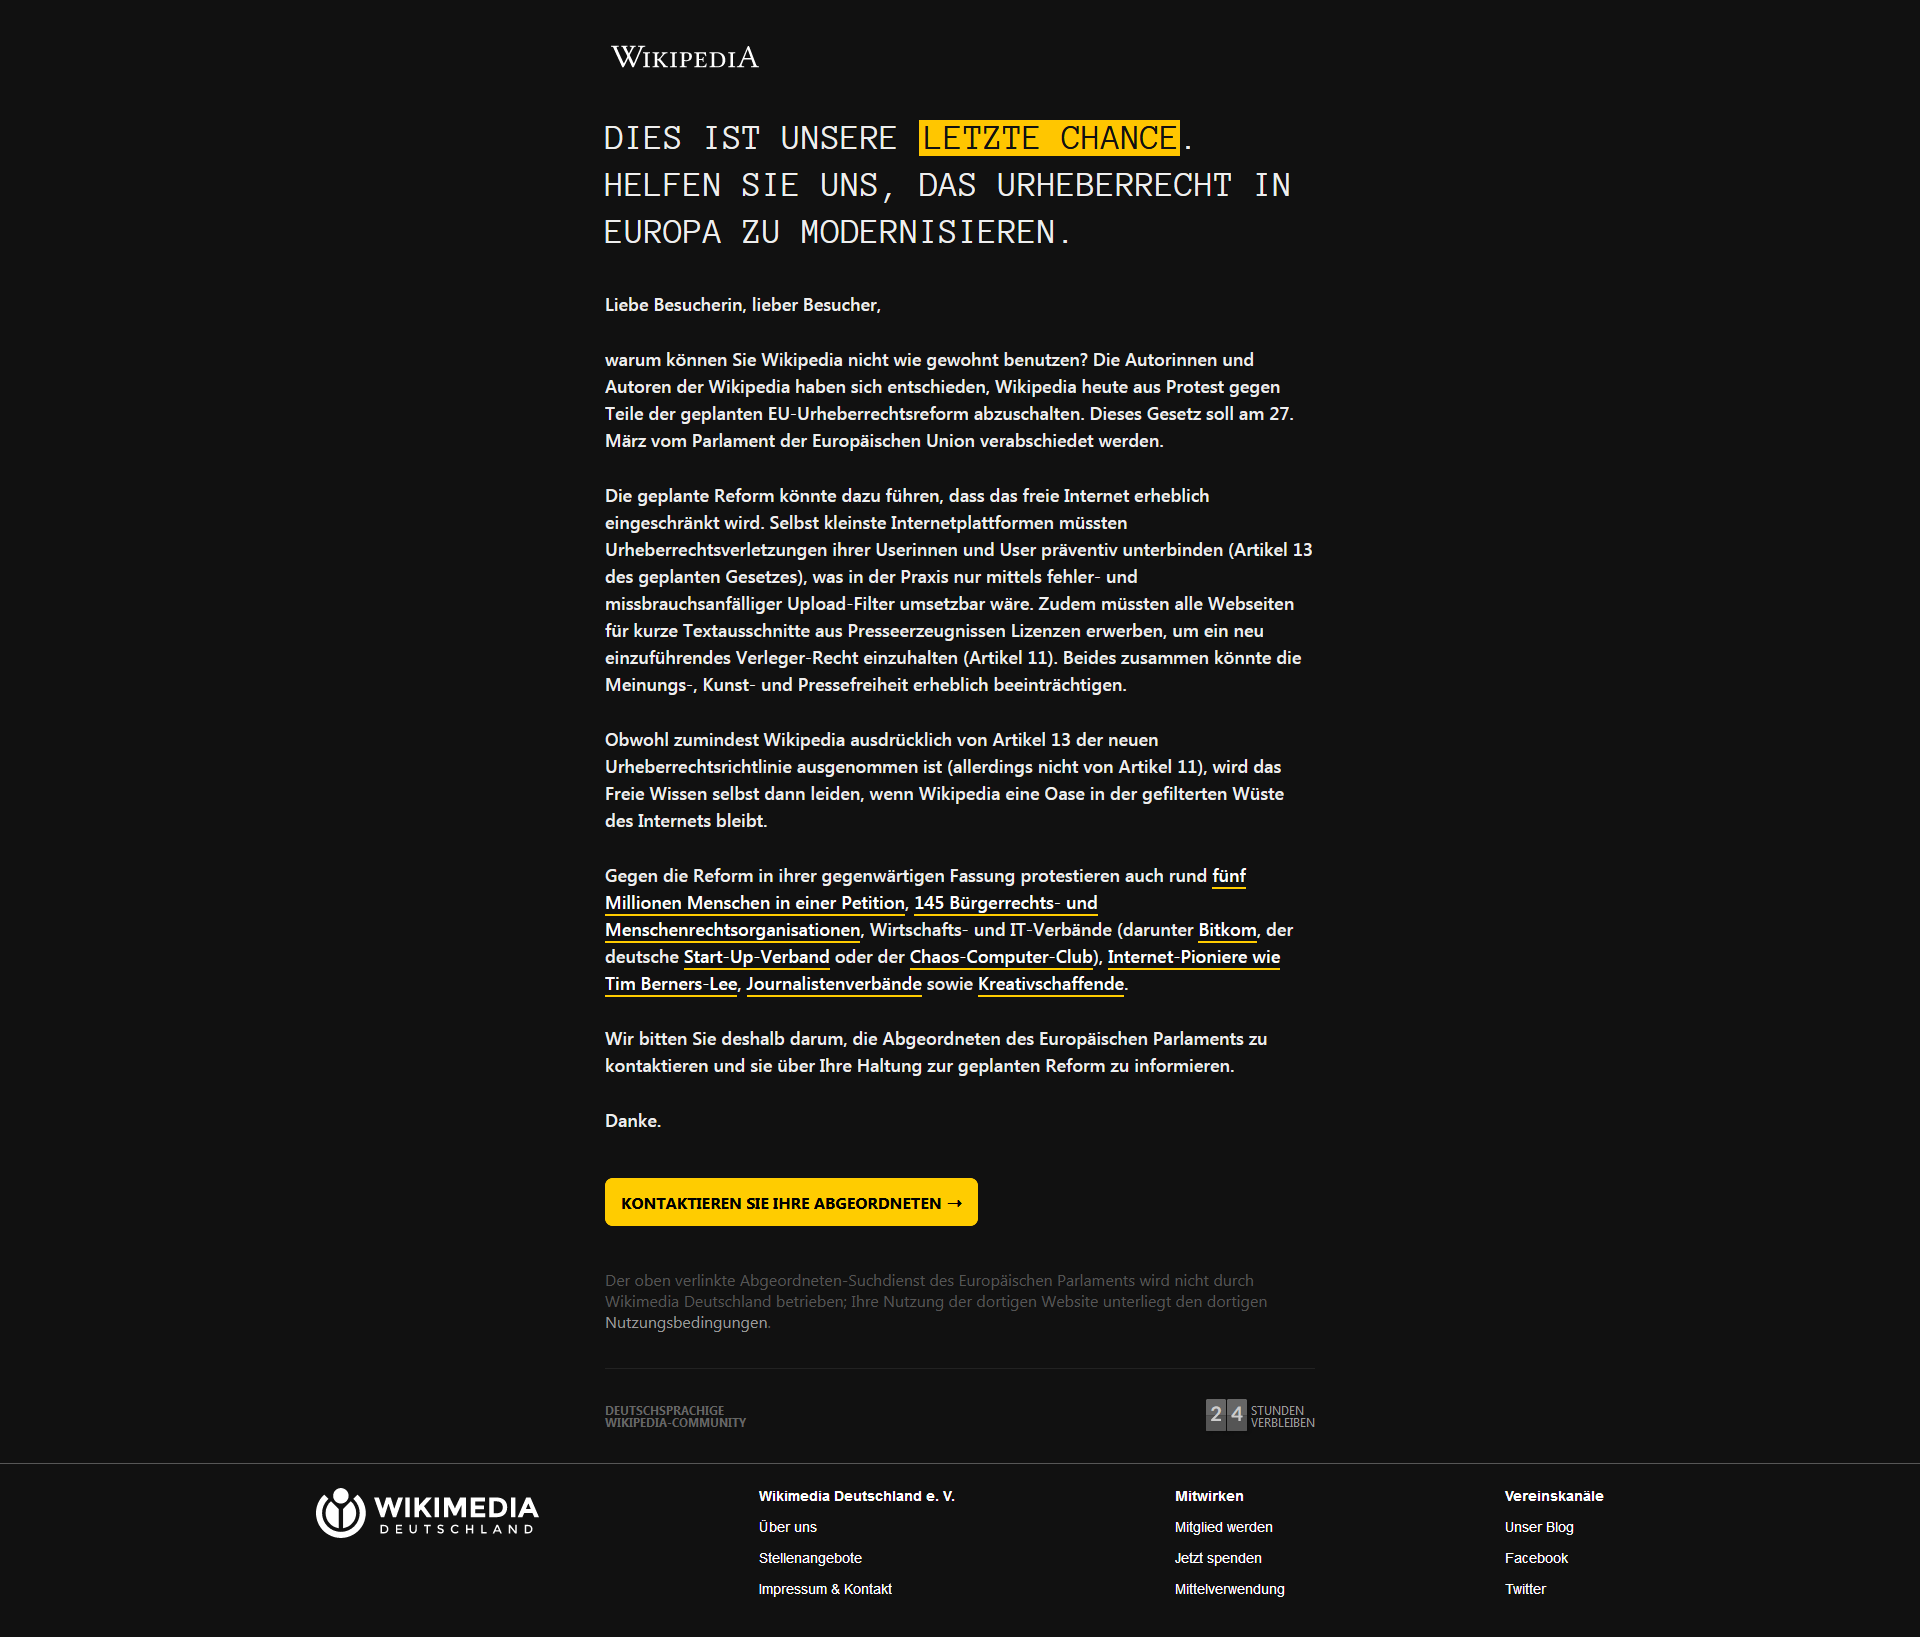
\includegraphics[width=0.9\columnwidth]{pics/Blackout_of_wikipediade_by_Wikimedia_Deutschland_-_March_2019.png}
  \caption{Blackout of wikipedia.de by Wikimedia Deutschland}~\label{fig:blackout-upload-filters}
\end{figure}

via
\url{https://de.wikipedia.org/wiki/Abschaltung_der_deutschsprachigen_Wikipedia_am_21._M%C3%A4rz_2019#/media/File:Blackout_of_wikipedia.de_by_Wikimedia_Deutschland_-_March_2019.png}

see also
\url{https://wikimediafoundation.org/2019/03/20/four-wikipedias-to-black-out-over-eu-copyright-directive/}
"Volunteer editor communities in four language Wikipedias—German, Czech, Danish, and Slovak—have decided to black out the sites on 21 March in opposition to the current version of the proposed EU Copyright Directive.

Those language editions of Wikipedia will redirect all visitors to a banner about the directive, blocking access to content on Wikipedia for 24 hours. "
"These independent language communities decided to black out in the same way most decisions are made on Wikipedia—through discussion and consensus, "

and
\url{https://wikimediafoundation.org/2019/02/28/we-do-not-support-the-eu-copyright-directive-in-its-current-form-heres-why-you-shouldnt-either/}

timeline
\url{https://edri.org/upload-filters-status-of-the-copyright-discussions-and-next-steps/}

\url{https://en.wikipedia.org/wiki/Directive_on_Copyright_in_the_Digital_Single_Market#Positions}

Interesting fact: there are edit filters that try to precisely identify the upload of media violating copyrights

%TODO refer to Lessig, Chapter 10 when making the upload filter commentary

\section{Directions for further studies}
<insert long list of interesting questions here>

\begin{itemize}
	\item Die Zusammenfassung sollte das Ziel der Arbeit und die zentralen Ergebnisse beschreiben. Des Weiteren sollten auch bestehende Probleme bei der Arbeit aufgezählt werden und Vorschläge herausgearbeitet werden, die helfen, diese Probleme zukünftig zu umgehen. Mögliche Erweiterungen für die umgesetzte Anwendung sollten hier auch beschrieben werden.
\end{itemize}
